%% latex-resume
%%
%% Copyright (c) 2012 Benjamin Coudrin <benjamin.coudrin@gmail.com>
%%                All Rights Reserved
%%
%%
%% This program is free software. It comes without any warranty, to
%% the extent permitted by applicable law. You can redistribute it
%% and/or modify it under the terms of the Do What The Fuck You Want
%% To Public License, Version 2, as published by Sam Hocevar. See
%% http://sam.zoy.org/wtfpl/COPYING for more details.
%%

\documentclass[11pt,a4paper]{article}%

% Packages
\usepackage[colorlinks, breaklinks, pdftitle={Benjamin Coudrin},pdfauthor={Coudrin, Benjamin}]{hyperref}%
\usepackage{xunicode}%
\usepackage{xltxtra}%
\usepackage{graphics}%
%\defaultfontfeatures{Mapping=tex-text}
\setmainfont[Mapping=tex-text]{Calluna}

\usepackage{tikz}
\usepackage{color}
\usepackage{array}

% Custom commands
\newcommand{\old}[1]{\fontspec[Alternate=1,Ligatures={Common, Rare}]{Calluna}\fontsize{24pt}{30pt}\selectfont #1}%

% Custom colors
\definecolor{orange}{RGB}{227,108,10}

% Let's start ...
\begin{document}%
\thispagestyle{empty}%

% Contacts watermark
\begin{tikzpicture}[remember picture,overlay]
	\node [scale=4,text opacity=0.15,xshift=1.55cm,yshift=-0.4cm] at (current page.north west) {\old contacts};
\end{tikzpicture}

% Contacts
\begin{tabular}{lcl}
	\multicolumn{1}{c}{\color{orange} 1.0}                               &  & \multicolumn{1}{c}{\color{orange} 2.0} \\
	                                                                     &  &                                        \\
	83 av. de Lespinet, 31400 Toulouse                                   &  & test                        \\
	{\color{orange} Tel.} 06.09.11.00.83                                 &  & test                        \\
	\href{mailto:benjamin.coudrin@gmail.com}{benjamin.coudrin@gmail.com} &  & test                        \\
	{\color{orange} born} 09/18/1983                                     &  & test                        \\
\end{tabular}

% Photo
\setlength{\fboxsep}{0pt}
\begin{tikzpicture}[remember picture,overlay]
	\node [xshift=-2.6cm,yshift=-2.6cm] at (current page.north east) {\fbox{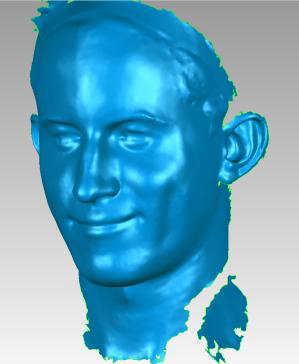
\includegraphics[height=4.3cm]{photo_3d}}};
\end{tikzpicture}

\end{document}%
